\documentclass[10pt,a4paper]{article}
\usepackage[latin1]{inputenc}
\usepackage{amsmath}
\usepackage{amsfonts}
\usepackage{amssymb}
\usepackage{graphicx}
\usepackage{float}

\begin{document}
\section*{Several Point Sources With Different Boundary Conditions}
When solving the Helmholtz equation with several point sources, it is possible to see the interference between the different sources. In figure \ref{fig:severalSourcesDBC3D} the two sources are located in (-0.25, -0.25) and (0.25, 0.25) with Dirichlet boundary conditions. We can see the constructive interference in the origin. The Robin boundary conditions will produce figure \ref{fig:severalSourcesRBC2D} and figure \ref{fig:severalSourcesRBC3D}. Here the point sources are located in (-0.25, -0.25), (0.50, 0.50) and (0.75, 0.75). The interference is clearly shown here as well, and we can see the middle peak's intensity is larger than at the location of the other sources.

\subsection*{Dirichlet Boundary Condition}
\begin{figure}[H]
\centering
    \includegraphics[width=0.9\textwidth]{figures/TwoSources_Dir3D.eps}
	\caption{Two point sources with Dirichlet boundary conditions plotted on the unit box.}
  \label{fig:severalSourcesDBC3D}
\end{figure}

\subsection*{Robin Boundary Condition}

\begin{figure}[H]
\centering
    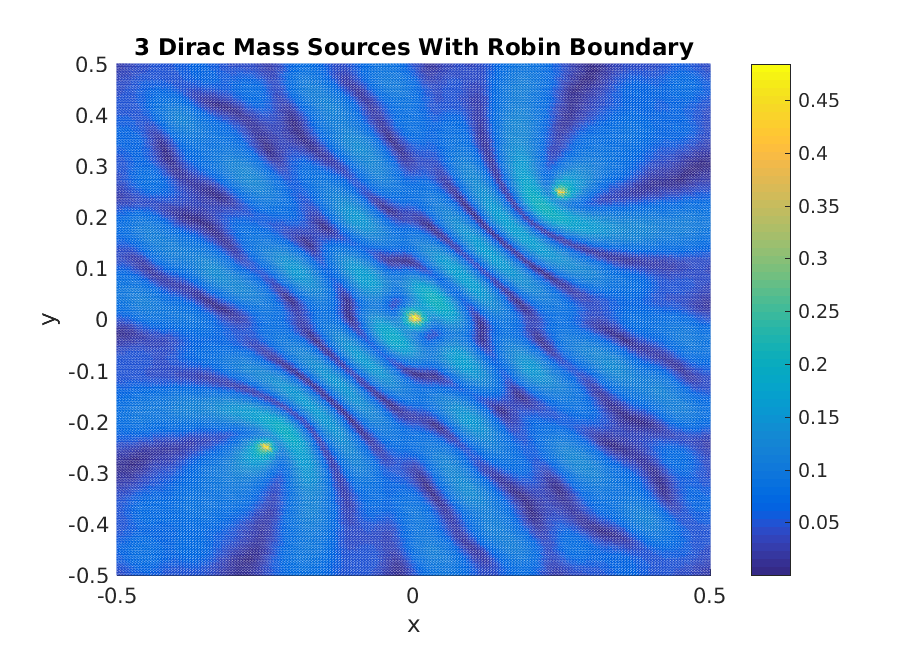
\includegraphics[width=0.8\textwidth]{figures/ThreeSources_2D.eps}
	\caption{Three point sources with Robin boundary conditions plotted on the unit box.}
  \label{fig:severalSourcesRBC2D}
\end{figure}

\begin{figure}[H]
\centering
    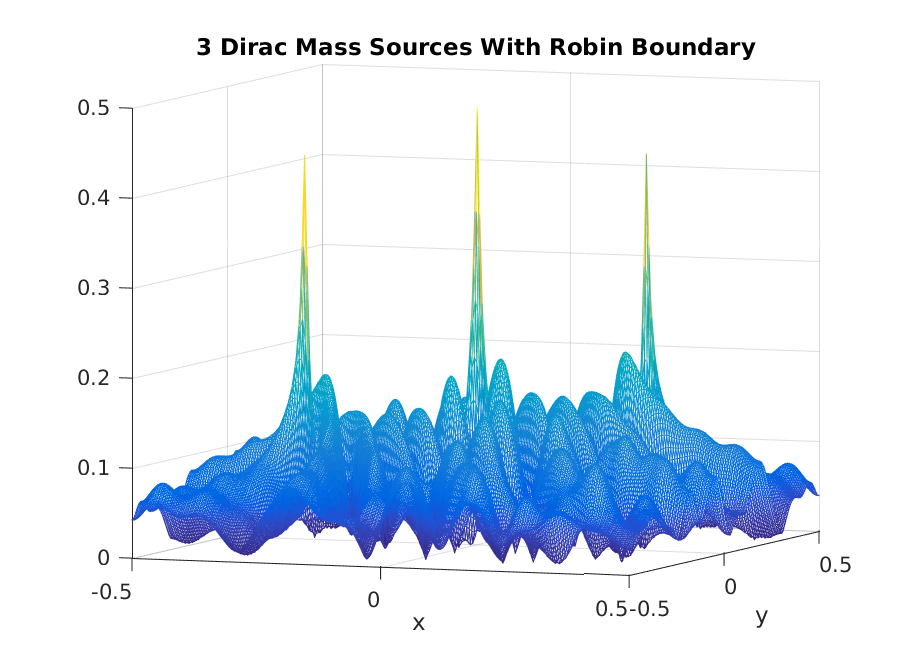
\includegraphics[width=0.8\textwidth]{figures/ThreeSources_3D.eps}
	\caption{Three point sources with Robin boundary conditions plotted on the unit box.}
  \label{fig:severalSourcesRBC3D}
\end{figure}

\end{document}